\chapter{磁力、矢量势与作用量原理}

\lectureoverview{静电力符合我们熟悉的保守力模式，但磁力依赖于速度。为了把它们纳入拉格朗日力学，我们首先发展所需的矢量微积分，利用磁场的无源性引入矢量势，考察其规范自由度，然后在作用量中构造磁力项。}

\section{一种新的力}

前面关于角动量、陀螺和泊松括号的讨论把若干主题联系在了一起。特别地，磁场中旋转的带电体会像陀螺一样进动。现在我们从这一类比转向单个带电粒子的运动。

静电力不需要新的力学。若\(U(\mathbf x)\)是势能，则
\begin{equation}
  \mathbf F=-\nabla U(\mathbf x),
\end{equation}
而通常的论证给出动能加势能守恒。对于电荷为\(e\)、处于静电势\(V(\mathbf x)\)中的粒子，
\begin{equation}
  U(\mathbf x)=eV(\mathbf x),
  \qquad
  \mathbf F_{\mathrm{el}}=-e\nabla V.
\end{equation}
磁力具有不同的形式。它们依赖于粒子的速度，因此不能仅仅通过再添加一个普通势能来引入。尽管如此，它们确实来自作用量原理，并且既有拉格朗日描述也有哈密顿描述。要达到这一描述，需要在矢量微积分中作一段简短但必不可少的插曲。

\section{场与局域操作}

\subsection{场记录了什么}

场为空间中的每一点、并且一般地为每一时刻指定一个物理量。温度和压强是标量场。风速是矢量场。电场和磁场是矢量场。其他理论即使在微观尺度上也包含标量场，而引力则由张量场描述。在目前的讨论中，我们略去任何时间依赖，把场写成\(\mathbf x\)的函数。

场的操作意义在于局域性。设想某个区域被藏在一个袋子里。要测量该区域内的电场，就在那里放一个小的检验电荷并观察它的加速度。力由电荷所在处的场决定，而不是通过与每一个远处源分别商议来决定。同样的说法适用于磁场和运动的检验电荷。稍后，矢量势将迫使我们对这一简单图像加以限定，但它是恰当的出发点。

\subsection{导数算符}

导数把场变成其他场。我们把三个空间导数收集成
\begin{equation}
  \nabla
  =
  \left(
    \frac{\partial}{\partial x},
    \frac{\partial}{\partial y},
    \frac{\partial}{\partial z}
  \right).
\end{equation}
这个符号读作\emph{del}或\emph{nabla}。它倒置三角形的样子令人印象深刻，但它真正的意义在于其行为在形式上像一个矢量，其分量是微分算符。

这是普通的三维物理空间，不是相空间，也不是多粒子位形空间。此外，\(\nabla\)不是一个可以单独存在的矢量场。它必须作用于某物。若\(T(\mathbf x)\)是标量温度场，则
\begin{equation}
  \nabla T
  =
  \left(
    \frac{\partial T}{\partial x},
    \frac{\partial T}{\partial y},
    \frac{\partial T}{\partial z}
  \right)
\end{equation}
是它的梯度，一个真正的矢量场。

\begin{figure}[htbp]
\centering
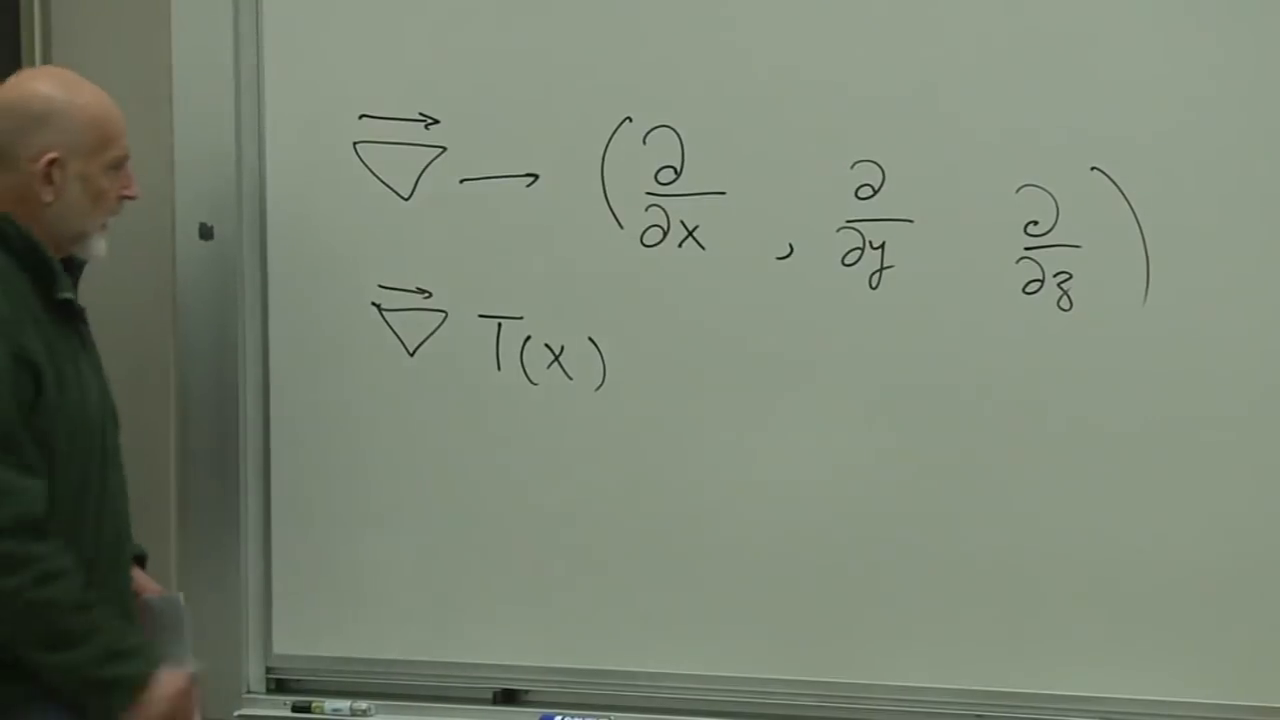
\includegraphics[width=0.82\textwidth]{lecture_09_figure_01.png}
\caption{黑板上引入\(\nabla\)作为空间导数算符的矢量，并开始把它作用于标量场\(T(\mathbf x)\)。}
\lectureframe{00:11:30}
\end{figure}

标量不仅仅是用一个分量写出的量。它是一个其值不依赖于坐标轴取向的量。温度是标准的例子。给定矢量场\(\mathbf E\)，局域表达式\(\mathbf E\cdot\mathbf E\)也是标量。相比之下，通过积分一个场来构造势是非局域操作；它使用沿路径的值。

\subsection{散度}

对于矢量场\(\mathbf A=(A_x,A_y,A_z)\)，标量
\begin{equation}
  \nabla\cdot\mathbf A
  =
  \frac{\partial A_x}{\partial x}
  +\frac{\partial A_y}{\partial y}
  +\frac{\partial A_z}{\partial z}
\end{equation}
是它的散度。用流体的语言说，正散度衡量局部向外流动的趋势，而负散度衡量向内汇聚的趋势。流体的源产生正散度；汇产生负散度。这一图像是定性的，但它将使磁场的无源性变得透明。

\section{叉积、epsilon符号与旋度}

\subsection{分量形式的叉积}

对于两个矢量 \(\mathbf V\) 和 \(\mathbf A\)，叉积的一个分量为
\begin{equation}
  (\mathbf V\times\mathbf A)_x
  =
  V_yA_z-V_zA_y.
\end{equation}
另外两个分量可通过循环 \(x\to y\to z\to x\) 得到。将 \(x,y,z\) 替换为指标 \(1,2,3\) 是有用的。克罗内克符号为
\begin{equation}
  \delta_{ij}
  =
  \begin{cases}
    1,&i=j,\\
    0,&i\ne j,
  \end{cases}
\end{equation}
而列维--奇维塔符号定义为
\begin{equation}
  \epsilon_{123}=\epsilon_{231}=\epsilon_{312}=1,
  \qquad
  \epsilon_{132}=\epsilon_{321}=\epsilon_{213}=-1,
\end{equation}
当任意两个指标重合时 \(\epsilon_{ijk}=0\)。围绕一个三小时钟面的循环顺序给出正号；反转方向则给出负号。交换任意一对指标会改变符号，因此 \(\epsilon_{ijk}\) 是完全反对称的。

我们还使用求和约定：在一个项中重复出现的指标从 \(1\) 到 \(3\) 求和。三个叉积方程于是变为
\begin{equation}
  (\mathbf V\times\mathbf A)_i
  =
  \epsilon_{ijk}V_jA_k.
\end{equation}
例如，令 \(i=1\) 则只剩下 \((j,k)=(2,3)\) 和 \((3,2)\)：
\begin{equation}
  (\mathbf V\times\mathbf A)_1
  =
  \epsilon_{123}V_2A_3
  +\epsilon_{132}V_3A_2
  =
  V_2A_3-V_3A_2.
\end{equation}
因此，这种紧凑记法恰好包含了熟悉的份量规则。

\subsection{伪装成反对称矩阵的矢量}

还有第二种表示：
\begin{equation}
  V_iA_j-V_jA_i
  =
  \epsilon_{ijk}(\mathbf V\times\mathbf A)_k.
\end{equation}
左边有两个指标，并且在 \(i\leftrightarrow j\) 下是反对称的。作为矩阵，它具有如下形式
\begin{equation}
  M_{ij}
  =
  \begin{pmatrix}
    0&M_{12}&M_{13}\\
    -M_{12}&0&M_{23}\\
    -M_{13}&-M_{23}&0
  \end{pmatrix}.
\end{equation}
对角线元素为零，下三角由上三角确定。因此有三个独立分量。

\begin{figure}[htbp]
\centering
\includegraphics[width=0.82\textwidth]{lecture_09_figure_02.png}
\caption{一个叉积分量以及用于计数其独立分量的示意性 \(3\times3\) 反对称阵列。单元格中的标记是助记性的，而非额外的符号。}
\lectureframe{00:34:20}
\end{figure}

\begin{classroomqa}
\audiencequestion{叉积，或者与另一个矢量的等同，在三维之外还有意义吗？}
\lecturerresponse{反对称的二指标对象在任何维度都有意义，但它与矢量的等同是三维所特有的。三维中的矢量有三个分量，而反对称的 \(3\times3\) 矩阵有三个独立分量。在四维中，相应的计数为四和六，因为 \(4(4-1)/2=6\)。反对称对象仍然存在，并且自然地被视为一个二形式，但它不是另一个四维矢量。}
\end{classroomqa}

\subsection{旋度}

将 \(\mathbf V\) 替换为 \(\nabla\) 定义了旋度：
\begin{equation}
  (\nabla\times\mathbf A)_i
  =
  \epsilon_{ijk}\frac{\partial A_k}{\partial x_j}.
\end{equation}
用通常的分量表示，
\begin{align}
  (\nabla\times\mathbf A)_x
  &=
  \frac{\partial A_z}{\partial y}
  -\frac{\partial A_y}{\partial z},\\
  (\nabla\times\mathbf A)_y
  &=
  \frac{\partial A_x}{\partial z}
  -\frac{\partial A_z}{\partial x},\\
  (\nabla\times\mathbf A)_z
  &=
  \frac{\partial A_y}{\partial x}
  -\frac{\partial A_x}{\partial y}.
\end{align}
散度衡量局部的发散，而旋度衡量局部的环流。绕轴旋转的流体沿该轴具有非零旋度。对于速度场，这一图像尤为生动，尽管该定义适用于任何矢量场。

\section{两个结构恒等式}

两个事实将完成几乎所有的数学工作：
\begin{equation}
  \nabla\cdot(\nabla\times\mathbf A)=0,
  \qquad
  \nabla\times(\nabla s)=0.
\end{equation}
第一个成立是因为二阶导数是交换对称的，而 \(\epsilon_{ijk}\) 是反对称的：
\begin{equation}
  \nabla\cdot(\nabla\times\mathbf A)
  =
  \epsilon_{ijk}\partial_i\partial_j A_k
  =0.
\end{equation}
第二个由混合偏导数的相等性得出：
\begin{equation}
  \bigl[\nabla\times(\nabla s)\bigr]_i
  =
  \epsilon_{ijk}\partial_j\partial_k s
  =0.
\end{equation}

\begin{figure}[htbp]
\centering
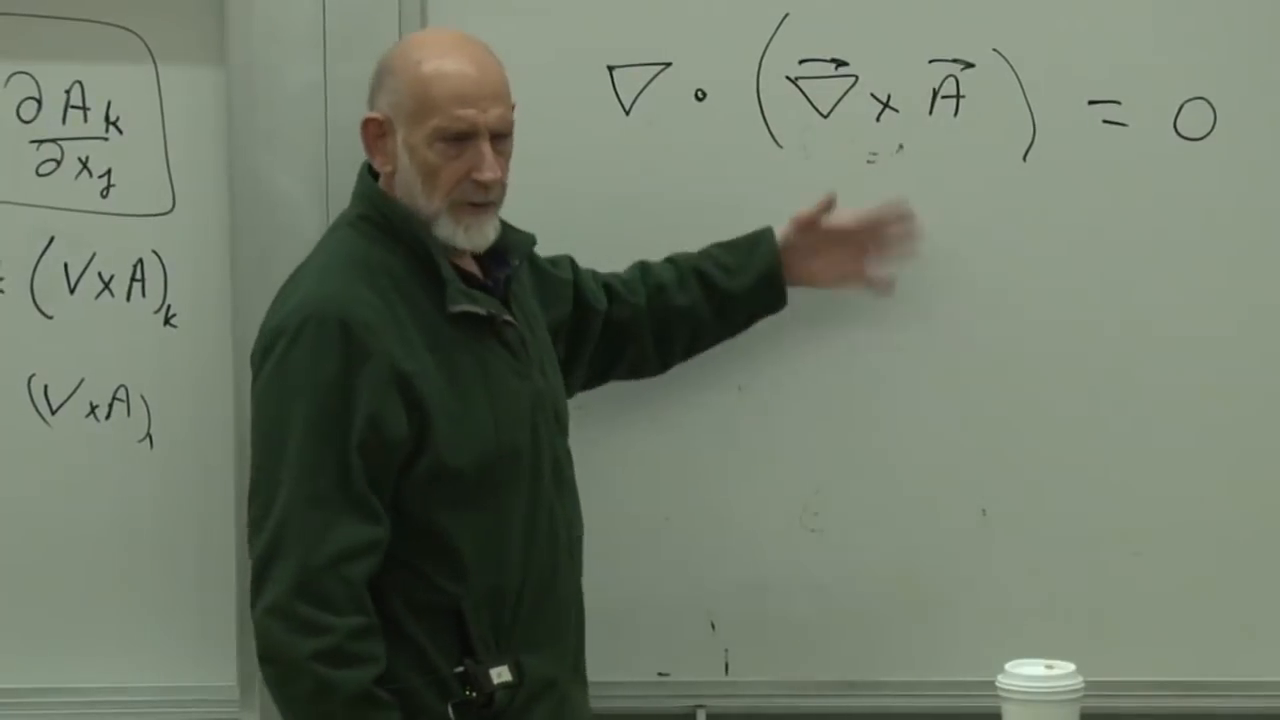
\includegraphics[width=0.80\textwidth]{lecture_09_figure_03.png}
\caption{黑板上的第一个恒等式：每个旋度的散度都为零。}
\lectureframe{00:38:26}
\end{figure}

这些是容易的方向，适合讲座承诺的作业或突击测验。逆命题需要更多小心。局部地，或在适当的单连通或可收缩区域上整体地，
\begin{align}
  \nabla\cdot\mathbf F=0
  &\quad\Longrightarrow\quad
  \mathbf F=\nabla\times\mathbf A,\\
  \nabla\times\mathbf F=0
  &\quad\Longrightarrow\quad
  \mathbf F=\nabla s.
\end{align}
没有区域条件的限定，洞和其他整体拓扑特征可能阻碍这些结论。讲座使用的是局部形式，这正是下文所需要的。

\section{为什么磁场是一个旋度}

\subsection{没有观测到的磁源}

磁场 \(\mathbf B\) 通过其对带电粒子和电流的作用在操作上被定义。在没有磁单极子的通常电磁学中，
\begin{equation}
  \nabla\cdot\mathbf B=0.
\end{equation}
这与电场不同，电场的散度正比于电荷密度。电荷是电通量的源和汇。尚未观测到磁通量的孤立源或汇。

磁单极子会改变这个方程。统一场论常常提供理论上的理由来预期这类对象，但如果它们存在，可能质量太大而无法在现有实验中产生。因此，当前理论在磁荷密度为零的情况下进行。

\begin{classroomqa}
\audiencequestion{磁单极子会是什么？普通磁体已经有北极和南极。}
\lecturerresponse{一个孤立的单极子将是磁场的真正源或汇，类似于电荷。普通的条形磁铁则不同。在其北极附近出现的场线弯曲穿过空间，并通过南极返回，继续穿过磁铁的材料。外部看起来是源和汇的东西是相连的，就像流体通过隐藏的管道流动。磁通量没有净的产生或消灭。}
\end{classroomqa}

\begin{figure}[htbp]
\centering
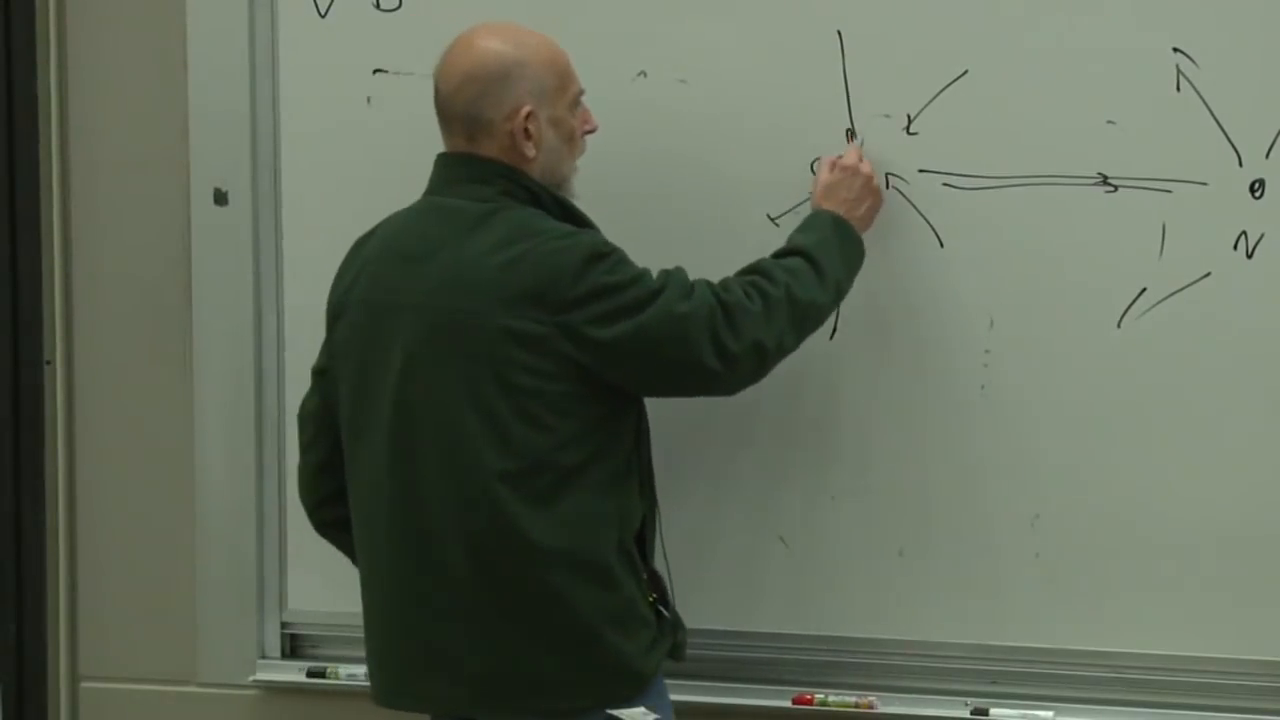
\includegraphics[width=0.76\textwidth]{lecture_09_figure_04.png}
\caption{黑板上将看似存在的北源与南源加以对照，同时让它们的场线通过磁体相连，从而强调磁通量并不在那里起始或终止。}
\lectureframe{00:44:56}
\end{figure}

由于\(\mathbf B\)无散度，逆定理允许我们至少局部地写出
\begin{equation}
  \boxed{\mathbf B=\nabla\times\mathbf A}.
\end{equation}
场\(\mathbf A\)就是矢势。乍看之下，这似乎只是对可测场\(\mathbf B\)的多余重述。其目的只有在我们构造作用量时才会变得清楚。

\subsection{矢势并不唯一}

若\(\mathbf A\)是一个矢势，则
\begin{equation}
  \mathbf A'=\mathbf A+\nabla s
\end{equation}
是另一个矢势，因为
\begin{equation}
  \nabla\times\mathbf A'
  =
  \nabla\times\mathbf A+\nabla\times(\nabla s)
  =
  \mathbf B.
\end{equation}
这种替换称为\emph{规范变换}。磁场是规范不变的。

\begin{figure}[htbp]
\centering
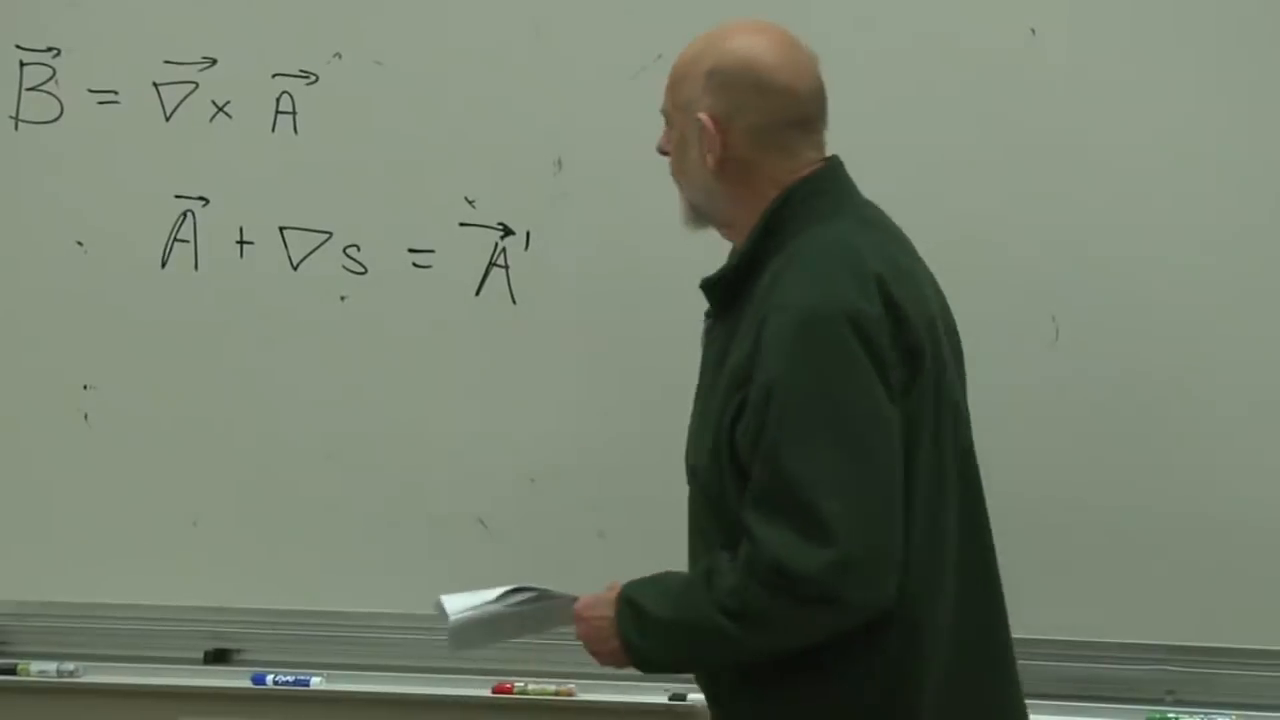
\includegraphics[width=0.80\textwidth]{lecture_09_figure_05.png}
\caption{定义关系\(\mathbf B=\nabla\times\mathbf A\)与规范移动\(\mathbf A'=\mathbf A+\nabla s\)一同出现在黑板上。}
\lectureframe{01:03:01}
\end{figure}

它的读音是\emph{gauge}，而不是\emph{gouache}或\emph{gouge}--——讲座以故作严厉的态度强调了这一区别。这个词本身是历史性的。它源于早期试图将这种自由度与不同地点长度标准的比较联系起来；那个原初解释没有留存下来，但名称留存了下来。

\begin{classroomqa}
\audiencequestion{在这一讨论中，规范变换是否特指\(\mathbf A\mapsto\mathbf A+\nabla s\)？}
\lecturerresponse{是的。这就是此处所使用的完整电磁变换。Yang--Mills理论及其他场论中的规范变换推广了同一思想，但电磁学只需要加上一个标量梯度。}
\end{classroomqa}

这种不唯一性也澄清了什么是可直接测量的。小区域中的带电粒子响应局域的\(\mathbf B\)，而所有由规范变换相联系的矢势在那里预言相同的力。不存在这种经典意义上的局域实验，能赋予\(\mathbf A\)一个唯一的值。

\begin{classroomqa}
\audiencequestion{加上一个梯度是否就是不唯一性的完整描述？}
\lecturerresponse{在简单区域上局部地看，是的。若\(\nabla\times\mathbf A'=\nabla\times\mathbf A\)，则\(\nabla\times(\mathbf A'-\mathbf A)=0\)，所以差是一个梯度。整体上，多连通区域可能带有额外的微妙之处。加上一个常矢量已经包含在内，因为常矢量是线性标量函数的梯度。给\(s\)本身加上一个常数不改变任何东西，因为它的梯度为零。}
\end{classroomqa}

\begin{classroomqa}
\audiencequestion{如果规范自由度有一个底层的物理原因，那是什么？}
\lecturerresponse{讲座推迟了那个更深的解释。有用的第一步是先处理这种自由度，并看看它如何进入作用量。一旦形式体系变得熟悉，规范描述为何不可或缺的原因就更容易辨认。}
\end{classroomqa}

\section{一个磁场，多个势}

考虑最简单的可能例子，
\begin{equation}
  \mathbf B=b\,\hat{\mathbf z},
  \qquad
  B_x=B_y=0,
  \qquad
  B_z=b,
\end{equation}
其中\(b\)是常数。一个矢势是
\begin{equation}
  \mathbf A^{(1)}=(0,bx,0).
\end{equation}
确实，
\begin{equation}
  (\nabla\times\mathbf A^{(1)})_z
  =
  \frac{\partial A_y^{(1)}}{\partial x}
  -\frac{\partial A_x^{(1)}}{\partial y}
  =b,
\end{equation}
而旋度的其他分量都为零。

这一选择似乎挑出了\(y\)方向，尽管物理场在\(x\)-\(y\)平面内具有旋转对称性。第二种选择使这种任意性变得明确：
\begin{equation}
  \mathbf A^{(2)}=(-by,0,0).
\end{equation}
它给出
\begin{equation}
  (\nabla\times\mathbf A^{(2)})_z
  =
  0-\frac{\partial(-by)}{\partial y}
  =b.
\end{equation}
两个势相差
\begin{equation}
  \mathbf A^{(2)}-\mathbf A^{(1)}
  =
  (-by,-bx,0)
  =
  \nabla(-bxy).
\end{equation}
因此它们是规范等价的。一个旋转对称的选择，
\begin{equation}
  \mathbf A^{(\mathrm{sym})}
  =
  \frac12\,\mathbf B\times\mathbf r
  =
  \left(-\frac{by}{2},\frac{bx}{2},0\right),
\end{equation}
是同一族中的另一个成员。

\begin{figure}[htbp]
\centering
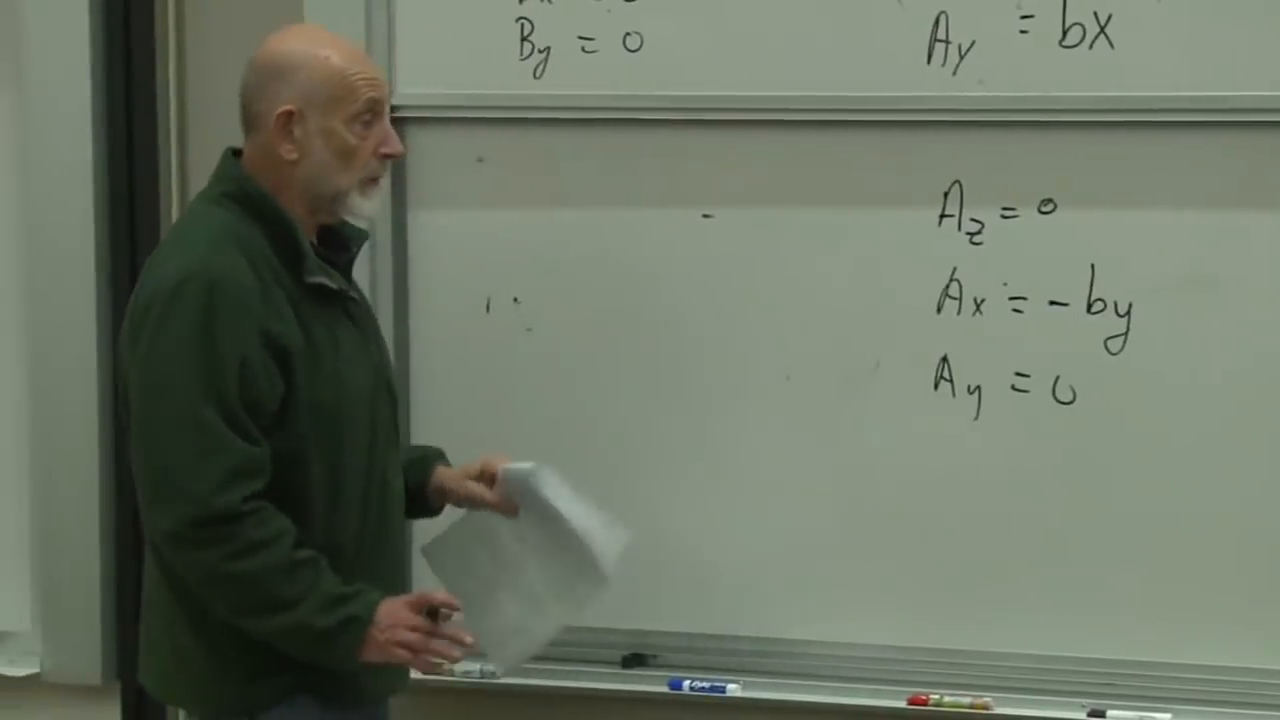
\includegraphics[width=0.80\textwidth]{lecture_09_figure_06.png}
\caption{两块黑板面板分别给出选择\(A_y=bx\)和\(A_x=-by\)，二者都产生相同的均匀场\(B_z=b\)。}
\lectureframe{01:07:20}
\end{figure}

\begin{classroomqa}
\audiencequestion{这与用不同方式安排载流线圈来产生场是同一种歧义吗？}
\lecturerresponse{不是。电流的不同安排是不同的物理源，即使它们在一个区域内一致，也可能在其他地方产生不同的场。在磁场处处被指定之后，规范自由度仍然存在：同一个物理的\(\mathbf B\)仍然有许多矢势。}
\end{classroomqa}

\begin{classroomqa}
\audiencequestion{能否把加上一个梯度想象成在不增加扭曲的情况下拉伸或压缩？}
\lecturerresponse{这是一个有用的几何直觉。旋度探测局部的扭曲部分，而纯梯度具有零旋度。这一陈述精确地编码在\(\nabla\times\nabla s=0\)中。}
\end{classroomqa}

\begin{classroomqa}
\audiencequestion{\(\mathbf A\)的方向与\(\mathbf B\)的方向之间是否存在固定的关系？}
\lecturerresponse{不存在任何与规范无关的关系。上述例子恰好有\(A_z=0\)，但可以加上一个常数\(A_z\)而不改变任何导数。那样\(\mathbf A\)就不再垂直于\(\mathbf B\)了。在这一经典讨论中，只有旋度具有不变的物理内容。}
\end{classroomqa}

在静电学中有一个较温和的类似情形。由于\(\mathbf E=-\nabla V\)，把\(V\)替换为\(V+C\)并不改变\(\mathbf E\)。选用\emph{矢势}这一术语，部分正是类比于普通标势中的这种自由度：人们可以以某种方式改变势，而物理场保持不变。

\section{洛伦兹力}

现在我们可以陈述作用量原理必须再现的力定律。在本书所用的约定下，
\begin{equation}
  \boxed{
  \mathbf F
  =
  e\left(
    \mathbf E+\frac{\mathbf v}{c}\times\mathbf B
  \right)
  =
  -e\nabla V+\frac{e}{c}\mathbf v\times\mathbf B
  }.
\end{equation}
符号\(e\)是粒子的电荷，\(\mathbf v=\dot{\mathbf x}\)是它的速度，\(V\)是标势。这一记号不应诱使我们把\(V\)与\(\mathbf v\)相混淆。用SI的语言说，\(V\)以伏特为单位，\(e\)以库仑为单位；所展示的\(1/c\)属于本讲所用的单位约定。结构上的要点与单位无关。

\begin{figure}[htbp]
\centering
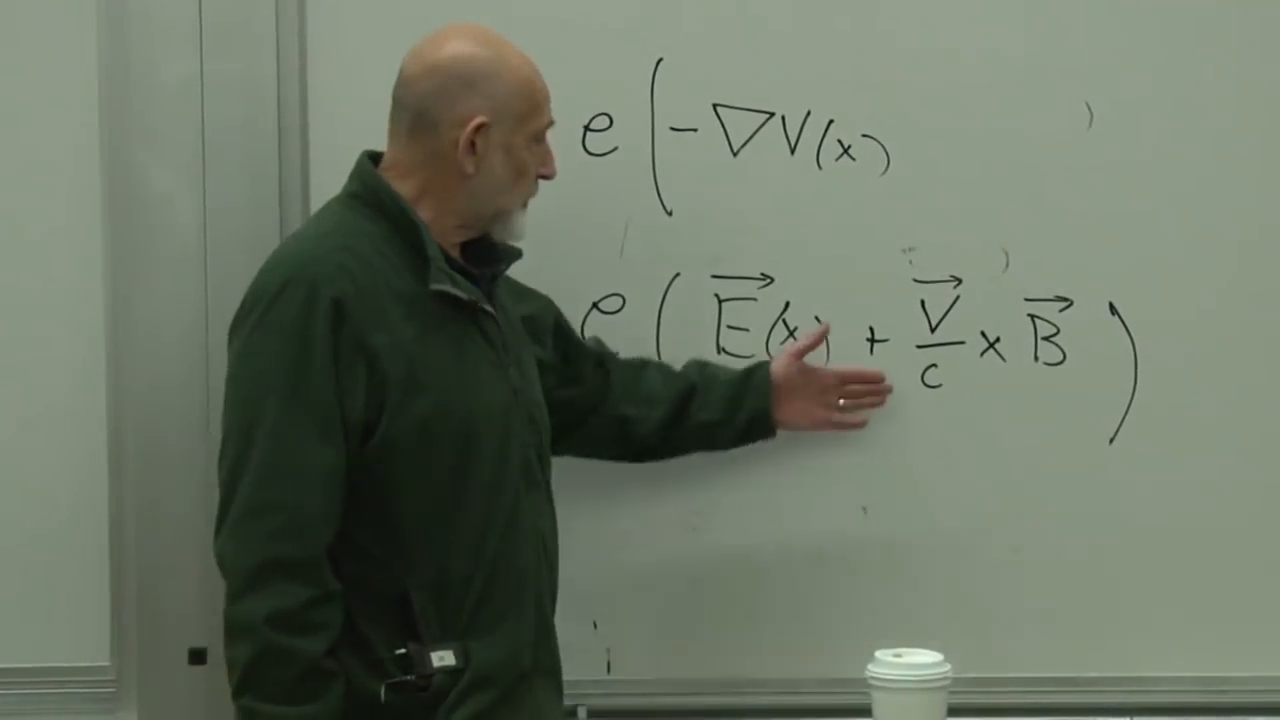
\includegraphics[width=0.82\textwidth]{lecture_09_figure_07.png}
\caption{洛伦兹力的电项与磁项被一并展示。磁的贡献正比于\(\mathbf v\times\mathbf B\)。}
\lectureframe{00:58:54}
\end{figure}

电项是保守的，并且已经熟悉。磁项则是新的。它对静止粒子为零，并且同时垂直于\(\mathbf v\)和\(\mathbf B\)。因此，
\begin{equation}
  \mathbf v\cdot\mathbf F_{\mathrm{mag}}
  =
  \frac{e}{c}\mathbf v\cdot(\mathbf v\times\mathbf B)
  =0.
\end{equation}
静磁场使轨迹弯曲，但对粒子不做功。这与黏性阻力不同，后者方向与速度相反，并会带走动能。

因子\(v/c\)也表明，在这些约定下，对于可比的场尺度，缓慢运动的粒子的磁效应往往小于电效应。电子足够轻，可以达到很大的速率，因此磁偏转仍然容易观察到。

历史上，人们先知道载流导线所受的力，后来才分离出单个电荷所受的力。洛伦兹认识到，通过把依赖于速度的项赋予每个运动电荷，就可以理解导线所受的力。完整的电加磁表达式现在被称为洛伦兹力定律，尽管在当前的讨论中磁的部分才是新颖之处。

\begin{classroomqa}
\audiencequestion{整个表达式有单独的符号吗，还是只有磁的部分才是洛伦兹力？}
\lecturerresponse{整个表达式就是力\(\mathbf F=m\mathbf a\)，它通常被称为洛伦兹力。磁项是历史上与洛伦兹联系最直接的部分。电场与磁场通过相对论有着深刻的联系，但当前的力学问题并不需要这种统一。}
\end{classroomqa}

\subsection{科里奥利类比}

我们以前见过速度与一个固定矢量叉乘。在以角速度\(\boldsymbol\omega\)转动的参考系中，科里奥利力可以写成
\begin{equation}
  \mathbf F_{\mathrm{Cor}}
  =
  2m\,\mathbf v\times\boldsymbol\omega.
\end{equation}
它与磁力具有相同的代数形式：
\begin{equation}
  2m\boldsymbol\omega
  \quad\longleftrightarrow\quad
  \frac{e}{c}\mathbf B.
\end{equation}
因此，垂直于平面的匀强磁场使带电粒子轨迹弯曲的方式，与转动参考系使运动物体偏转的方式大致相同。

\begin{figure}[htbp]
\centering
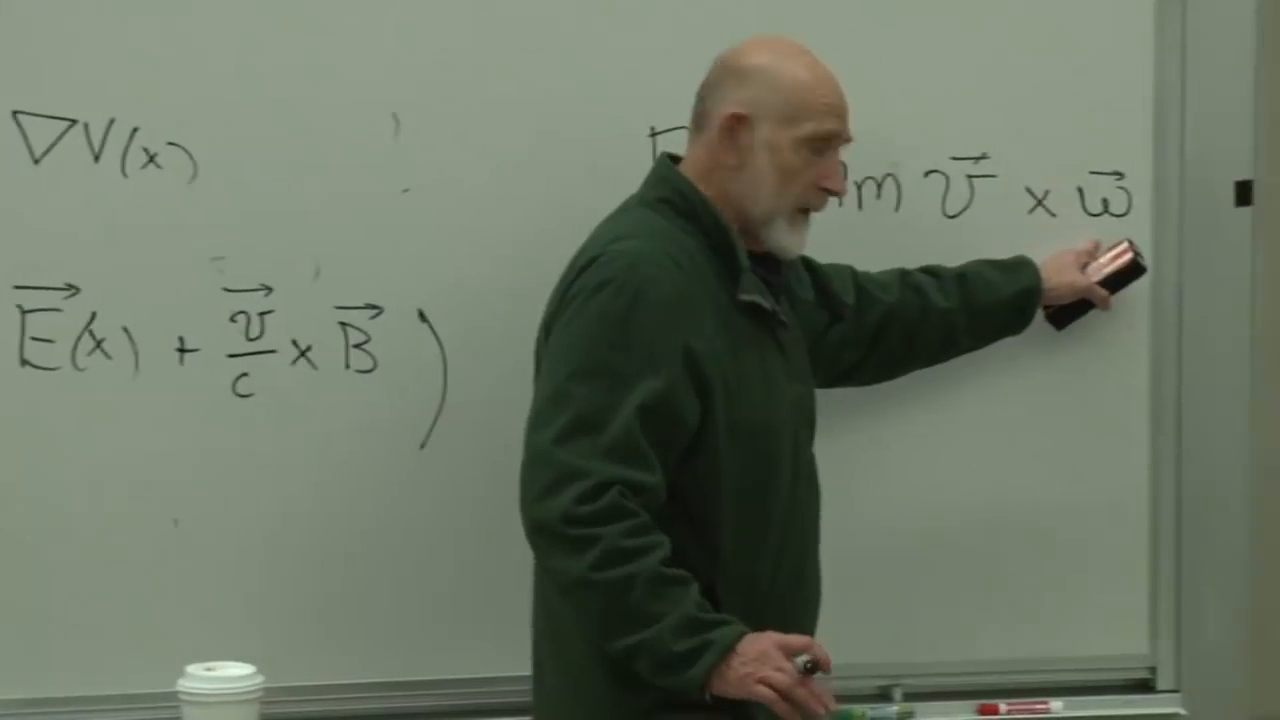
\includegraphics[width=0.82\textwidth]{lecture_09_figure_08.png}
\caption{洛伦兹力留在左边，而板书加上相应的科里奥利形式\(2m\,\mathbf v\times\boldsymbol\omega\)。}
\lectureframe{01:02:08}
\end{figure}

\begin{classroomqa}
\audiencequestion{科里奥利力被称为虚构力。它因为依赖于速度，就比磁力更不真实吗？}
\lecturerresponse{依赖于速度并不是问题所在。在转动平台上的人可以握住一个运动物体并感受到科里奥利力。它被称为虚构力，是因为它在惯性系中消失，而转动参考系恰恰由这类惯性项的存在来定义。\emph{真实}一词往往不如说明正在使用哪个参考系和哪个方程有用。}
\end{classroomqa}

这一类比可以推进为一个小的思想实验。在转动平台上，对于选定的粒子，适当的静电场可以抵消离心项，而适当的匀强磁场可以抵消科里奥利项。这种抵消只对选定的荷质比成立：电力和磁力按\(e\)标度，而惯性力按\(m\)标度。为电子调好的场配置，对于具有不同\(e/m\)的粒子，不会抵消同样的项。

\section{构造带电粒子的作用量}

\subsection{固定端点下的稳定作用量}

我们现在提出核心问题：洛伦兹力能否从作用量原理推导出来？答案是肯定的，但矢量势不可或缺。仅由粒子和\(\mathbf B\)局部构造的拉格朗日量无法产生所需的磁力。与其证明这一否定性结论，我们不如直接构造成功的作用量。

对于轨迹\(\mathbf x(t)\)，写出
\begin{equation}
  S[\mathbf x]
  =
  \int_{t_i}^{t_f}L(\mathbf x,\dot{\mathbf x},t)\,dt.
\end{equation}
讲义中作用量和矢量势使用了相同的手写字母，但我们用\(S\)表示作用量，用\(\mathbf A\)表示矢量势。物理路径在保持两端点固定的变分下使\(S\)取稳定值。传统说法\emph{最小作用量}虽然方便，但稳定作用量更为准确，因为极值不必是最小值。

固定端点很重要。可以想象路径的两端被钉在板上，而内部被来回拨动。这是普通力学中的轨迹，而非弦论对象；弦的图像只是将变分可视化的方式。

\subsection{拉格朗日量中可以包含什么？}

所有场都关闭时，拉格朗日量为动能，
\begin{equation}
  L_0=\frac{m}{2}\dot{\mathbf x}^{\,2}.
\end{equation}
静电项也是标准的：
\begin{equation}
  L_{\mathrm{el}}=-eV(\mathbf x).
\end{equation}
磁学项必须满足若干线索：
\begin{enumerate}
  \item 它必须与电荷\(e\)成正比；
  \item 它必须包含讲义单位制中的因子\(1/c\)；
  \item 它必须涉及速度；
  \item 它必须是一个旋转标量。
\end{enumerate}

诱人的尝试\(\mathbf B\cdot\dot{\mathbf x}\)是一个标量且包含速度，但它给出错误的运动方程。正确的项使用矢量势：
\begin{equation}
  L_{\mathrm{mag}}
  =
  \frac{e}{c}\mathbf A(\mathbf x)\cdot\dot{\mathbf x}
  =
  \frac{e}{c}A_i(\mathbf x)\dot x_i.
\end{equation}
因此完整的定态电磁拉格朗日量为
\begin{equation}
  \boxed{
  L
  =
  \frac{m}{2}\dot{\mathbf x}^{\,2}
  +\frac{e}{c}\mathbf A(\mathbf x)\cdot\dot{\mathbf x}
  -eV(\mathbf x)
  }.
\end{equation}
第10讲将应用欧拉--拉格朗日方程，并明确展示该表达式产生洛伦兹力。

\begin{figure}[htbp]
\centering
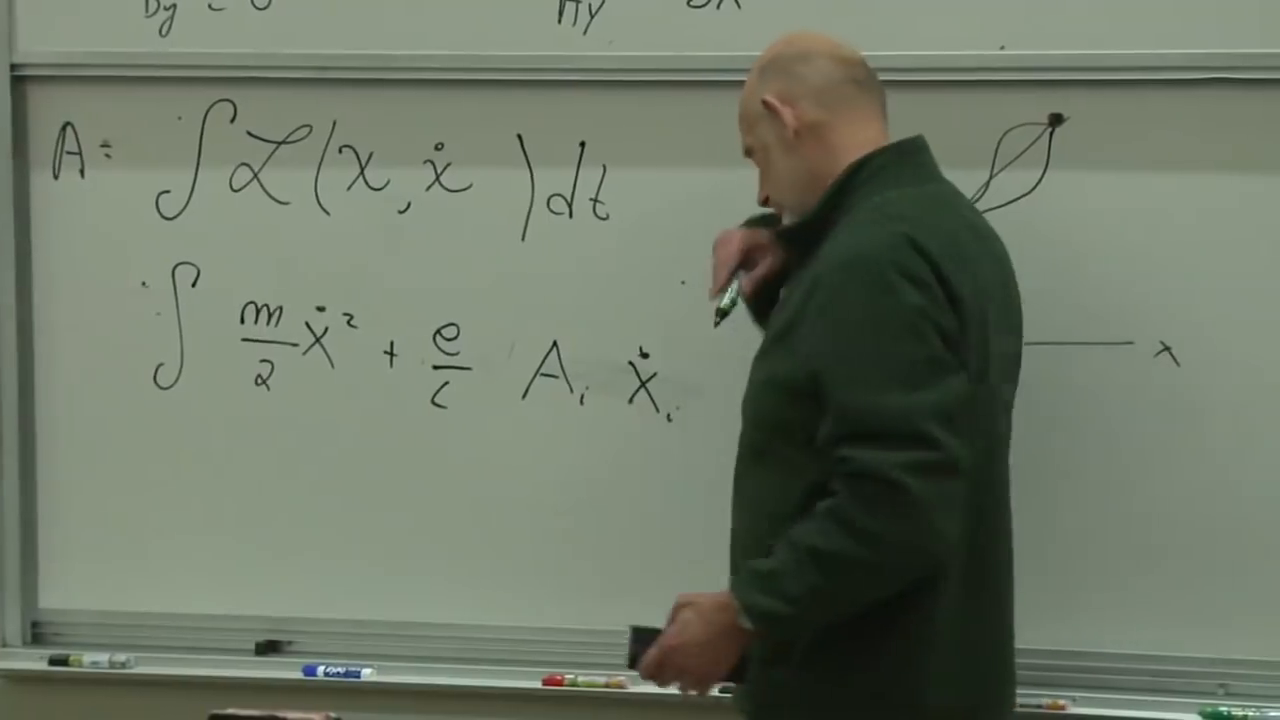
\includegraphics[width=0.82\textwidth]{lecture_09_figure_09.png}
\caption{作用量的完整板书构造：自由动能项加上\((e/c)A_i\dot x_i\)。}
\lectureframe{01:26:36}
\end{figure}

\section{规范变换只改变端点}

作用量中的磁学贡献为
\begin{equation}
  S_{\mathrm{mag}}
  =
  \frac{e}{c}
  \int_{t_i}^{t_f}A_i(\mathbf x)\dot x_i\,dt.
\end{equation}
由于\(\dot x_i\,dt=dx_i\)，它是沿粒子路径\(\gamma\)的线积分：
\begin{equation}
  S_{\mathrm{mag}}
  =
  \frac{e}{c}\int_\gamma A_i\,dx_i
  =
  \frac{e}{c}\int_\gamma\mathbf A\cdot d\mathbf x.
\end{equation}
将路径分成短线段，取\(\mathbf A\)沿每一线段的分量，乘以线段长度，再相加。这就是该积分的几何意义。

现在进行规范变换
\begin{equation}
  A_i\longmapsto A_i+\partial_i s.
\end{equation}
作用量的变化为
\begin{align}
  \Delta S
  &=
  \frac{e}{c}\int_\gamma \partial_i s\,dx_i\\
  &=
  \frac{e}{c}\int_\gamma ds\\
  &=
  \frac{e}{c}
  \left[
    s(\mathbf x_f)-s(\mathbf x_i)
  \right].
\end{align}
每个无穷小线段贡献\(s\)在一端的值减去在另一端的值。求和时，所有内部贡献发生望远镜式相消，只剩下两个端点。

\begin{figure}[htbp]
\centering
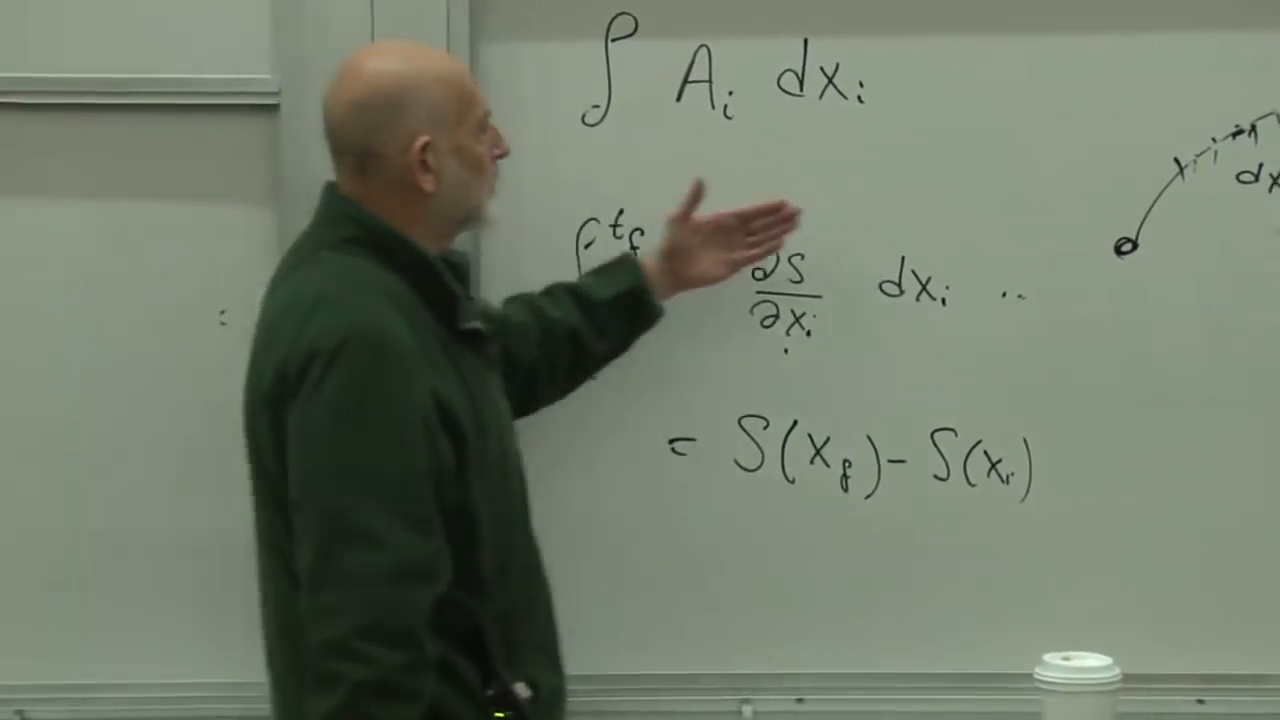
\includegraphics[width=0.82\textwidth]{lecture_09_figure_10.png}
\caption{线积分、其分割为小路径线段以及端点结果\(s(\mathbf x_f)-s(\mathbf x_i)\)。}
\lectureframe{01:32:31}
\end{figure}

\begin{classroomqa}
\audiencequestion{如果作用量在规范变换下改变，为什么轨迹不改变？}
\lecturerresponse{作用量原理比较的是具有固定初始点和最终点的路径。所添加的量只依赖于这些端点，因此对于比较中的每一条路径它都有相同的值。其变分为零。数值作用量并非严格不变，但欧拉--拉格朗日方程和物理轨迹是规范不变的。}
\end{classroomqa}

这一区分是本讲的主要概念性结果：
\begin{equation}
  \begin{aligned}
    S&\ \hbox{may shift by an endpoint term},\\
    \delta S&\ \hbox{and the equations of motion do not}.
  \end{aligned}
\end{equation}
因此规范自由度与作用量原理相容。矢量势可以进入拉格朗日量，尽管磁场并不选出唯一的\(\mathbf A\)。

\section{论证继续之处}

本讲已经组装了工具和作用量，但有意在变分该作用量之前停下。接下来的步骤现已确定：
\begin{enumerate}
  \item 应用欧拉--拉格朗日方程并恢复
  \(\mathbf F_{\mathrm{mag}}=(e/c)\mathbf v\times\mathbf B\)；
  \item 计算正则动量，它将不同于\(m\mathbf v\)；
  \item 构造哈密顿量；
  \item 确定守恒定律；
  \item 求解带电粒子在均匀磁场中的运动。
\end{enumerate}

通往这些结果的路径解释了为何引入矢量势。磁场是局部可测量的旋度，但矢量势才是与粒子路径自然耦合的对象。规范变换只在固定端点处改变这种耦合，力学保持不变。
